%!TEX root = ..\main.tex
\section{Model}
\label{sec:model}

\begin{figure*}[t]
\centering
	\includegraphics[width=0.9\textwidth]{Images/fullSystemPicture}
	\captionsetup{justification=centering, width=0.9\textwidth}
	\caption{Snapshot of for density $\rho = 0.95$ and $k_BT = 1.5$. Arrows represent the dipole moment of the particle. System sample obtained by means of Langevin dynamics simulation. The simulation was allowed to equilibrate for time $t = 100$ with fluid medium viscosity $\eta = 1$ and particle mass $m = 1$.}
	\label{fig:fullSystemPicture}
\end{figure*}

We consider colloidal particles with a permanent dipole moment $\mu \hat{m}$, where $\hat{m}$ is a unitary vector with the direction of the dipole moment. While considering a three-dimensional system, we constrain particle translational motion to a one-dimensional line, i.e. particles are confined to the $z$ axis. However, particles can explore the full three dimensional orientation space. Example of particle positions and orientations is given at \figref{fig:fullSystemPicture}.

The particle-particle interaction is described as the superposition of two contributions: a dipole-dipole interaction and a short-range repulsion.

The energy of dipole-dipole interaction for any pair (i, j) of particles is given by

\begin{equation}
\label{eq:dipole_dipole_interaction}
U^{dip}_{ij} =
	- \frac{\mu_i \mu_j}{\Delta r^3}[
		3 (\hat{m}_i \cdot \hat{r}_{ij})(\hat{m}_j \cdot \hat{r}_{ij})
		- (\hat{m}_i \cdot \hat{m}_j)
	]
\end{equation}
where $\mu_i \hat{m}_i$ and $\mu_j \hat{m}_j$ are dipole moments of interacting particles, $\vec{r}_{ij}$ is the direction vector which connects particle centers, and $\Delta r$ is the absolute value of the distance between particle centers.

By constraining particles to a 1D tube we effectively enforce $\vec{r}_{ij}$ to be co-aligned with $z$ axis. Assuming that all particles have the same dipole moment $\mu_i = \mu_j = \mu$, and defining $\mu = 1$ \textcolor{red}{meaning that the dipole moment is in units of "particle dipole moment"}, (\ref{eq:dipole_dipole_interaction}) can be simplified as:

\begin{equation}
\label{eq:dipole_dipole_1D}
E_{ij}^{dip} = - \frac{1}{\Delta z^3} [3 \cos \theta_i \cos \theta_j - (\hat{m}_i \cdot \hat{m}_j)]
\end{equation}
where $\theta_i$ and $\theta_j$ are the angles between $z$ axis and dipole moments of the first and second particle respectively, and $\Delta z = |z_j - z_i|$, where $z_i$ and $z_j$ are particle positions along $z$ axis.

The repulsive part is described by Yukawa potential
\begin{equation}
\label{eq:yukawa_interaction}
E_{ij}^{rep} = \frac{A \exp(-k \Delta z)}{\Delta z}
\end{equation}
where $A$ and $k^{-1}$ --- are the strength and range of interaction. \figref{fig:interaction_energy} show examples of $E_{ij}$ for different parameters.

\begin{figure}[p]
\centering
	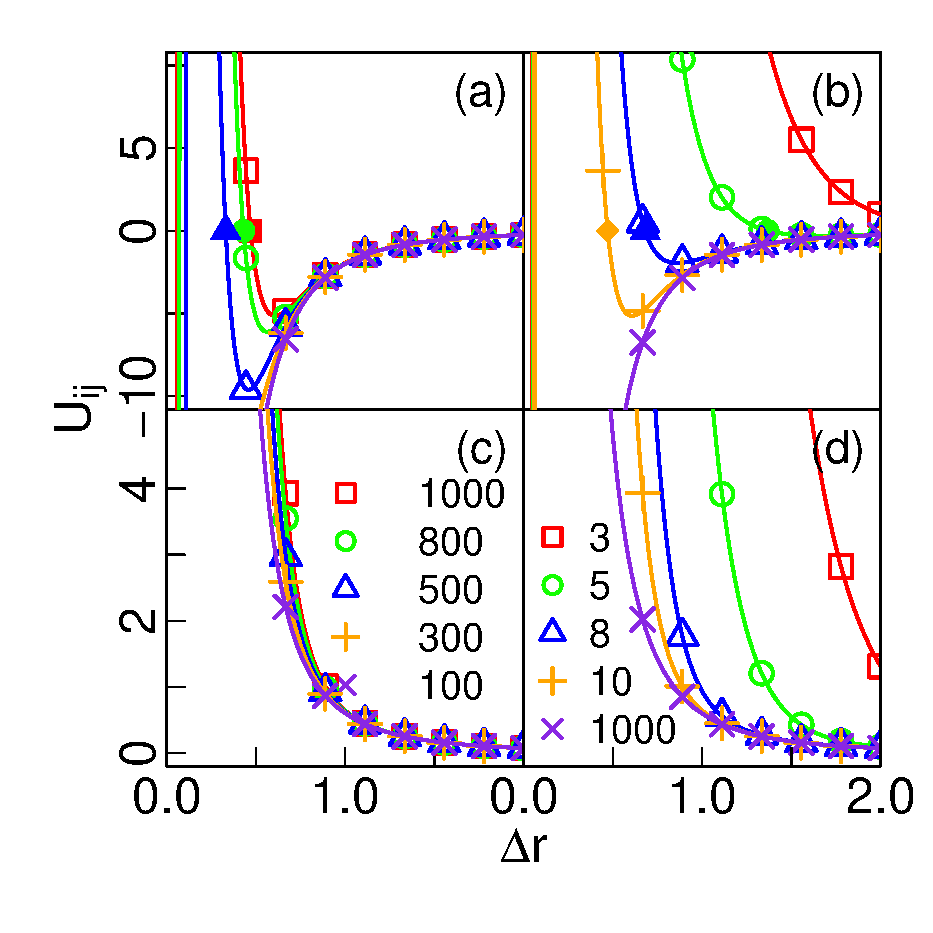
\includegraphics[width=0.9\textwidth]{Images/particle_interaction_potential}
\captionsetup{justification=centering, width=0.9\textwidth}
\caption{Potential energy as function of distance between centres of two interacting particles for co-aligned (top) and perpendicular (bottom) orientation of the particles dipole moments. Left plots show energy for the fixed value of $k = 10$, and right for the fixed value of $A = 1000$}
\label{fig:interaction_energy}
\end{figure}

When the dipole moments are perpendicular to each other the interaction is purely repulsive. However, as we can see on the \figref{fig:interaction_energy}(a) and \figref{fig:interaction_energy}(b), for low values of $A = 100$, combined with high values of $k = 10$, we can observe purely attractive interaction \textcolor{red}{The violet curve with diagonal crosses on the \figref{fig:interaction_energy}, it doesn't go up after it went down. So it's purely attractive}. Since in that case all particles will coalesce in one point, we assumed $A = 1000$ and $k = 10$, the case where interaction energy have well-defined minimum and maximum.
